\documentclass[11pt]{article}
    \title{\textbf{3. MĚŘENÍ NA NAPĚŤOVÉM DĚLIČI}}
    \author{Tomáš Kysela}
    \date{21/2/2022}
    
    \addtolength{\topmargin}{-3cm}
    \addtolength{\textheight}{3cm}
    
\usepackage[czech]{babel}
\usepackage{graphicx}
\begin{document}

\maketitle
\thispagestyle{empty}

\section{Úkol měření}
\begin{enumerate}
\item Změřte výstupní napětí $U_2$ děliče sestaveného z deseti rezistorů stejné jmenovité hodnoty pro všechny dělicí poměry $d$, a to:
   \begin{enumerate}
   \item číslicovým voltmetrem
   \item magnetoelektrickým voltmetrem (na rozsahu $12V$).
   \end{enumerate}
   Do společného grafu vyneste závislosti $U_2 /U_1 = f(d)$ a vysvětlete jejich rozdíly. Velikost napájecího napětí děliče $U_1 = 10 V$.
   
\item Z naměřených hodnot vypočtěte výstupní odporděliče $R_D$ pro zadaný dělicí poměrd za předpokladu, že vstupní odpor číslicového voltmetru se blíží k nekonečnu.

\item Vypočtěte \textbf{rozšířenou nejistotu typu B} (koeficient rozšíření $k_r = 2$), s jakou jste určili výstupní odpor děliče $R_D$ za předpokladu, že vnitřní odpor magnetoelektrického voltmetru je definován s tolerancí $0.2\%$.
\end{enumerate}
\section{Schéma zapojení}
\begin{figure}[htp]
\centering
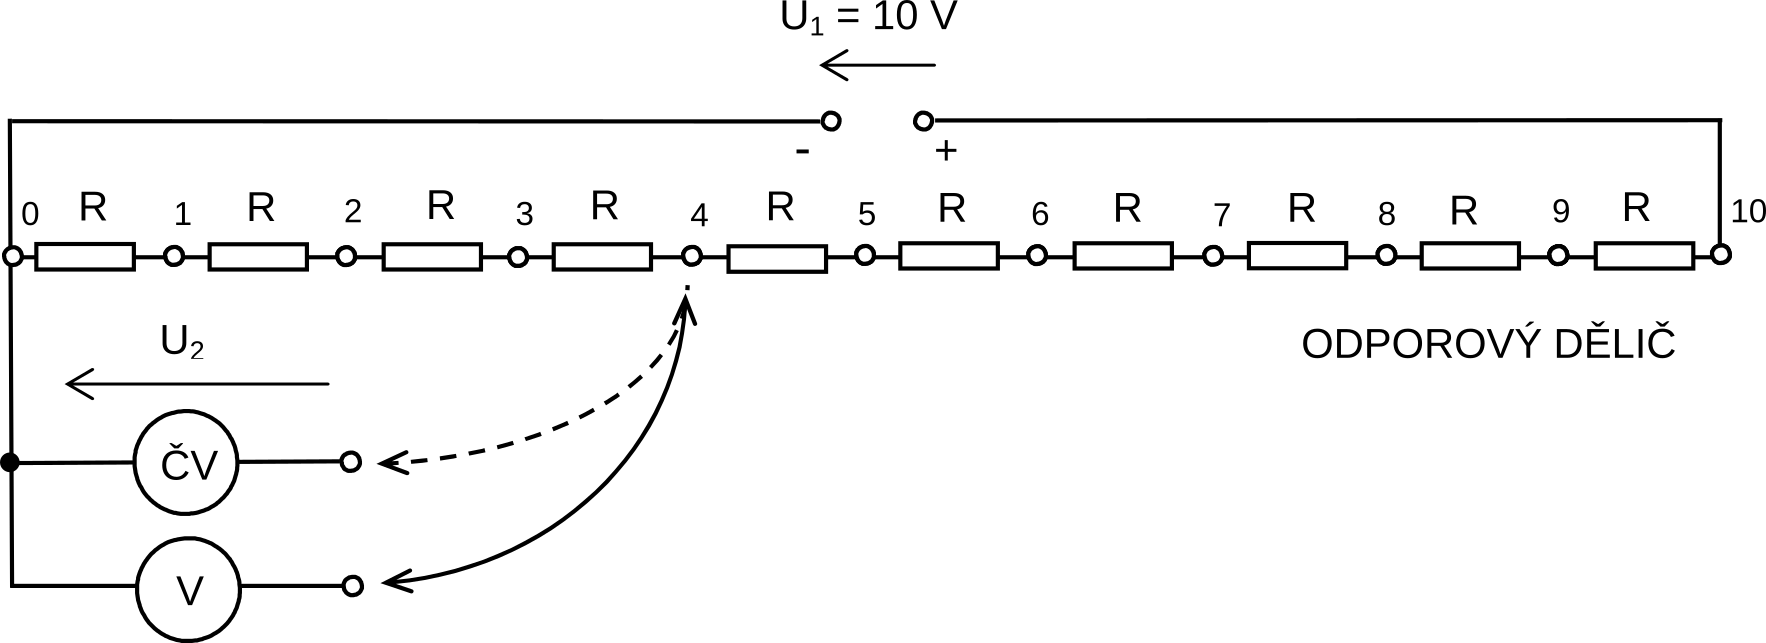
\includegraphics[scale=1.00]{LAB3.png}
\caption{Schéma zapojení}
\end{figure}
\section{Soupis použitých přístrojů}
\begin{tabular}{ll}
	V & voltmetr magnetoelektrický, tř.přes. $0.5$, rozsah $12 V$, odpor $500 \Omega/V$\\
	ČV & voltmetr číslicový, typ M1T 330, přesnost $\pm 0,01\%$ údaje $\pm 0,01\%$ rozsahu\\
	U1 & zdroj stejnosměrného napětí, typ AGILENT E3640A\\
	Př1 & odporový dělič
\end{tabular}

\section{Teoretický základ}

\begin{equation}
U_1 = U_2
\end{equation}

\end{document}

